%iffalse
\let\negmedspace\undefined
\let\negthickspace\undefined
\documentclass[journal,12pt,onecolumn]{IEEEtran}
\usepackage{cite}
\usepackage{amsmath,amssymb,amsfonts,amsthm}
\usepackage{algorithmic}
\usepackage{graphicx}
\usepackage{textcomp}
\usepackage{xcolor}
\usepackage{txfonts}
\usepackage{listings}
\usepackage{enumitem}
\usepackage{mathtools}
\usepackage{gensymb}
\usepackage{comment}
\usepackage[breaklinks=true]{hyperref}
\usepackage{tkz-euclide} 
\usepackage{gvv}                                        
%\def\inputGnumericTable{}                                 
\usepackage[latin1]{inputenc}     
\usepackage{xparse}
\usepackage{color}                                            
\usepackage{array}                                            
\usepackage{longtable}                                       
\usepackage{calc}                                             
\usepackage{multirow}
\usepackage{multicol}
\usepackage{hhline}                                           
\usepackage{ifthen}                                           
\usepackage{lscape}
\usepackage{tabularx}
\usepackage{array}
\usepackage{float}
\newtheorem{theorem}{Theorem}[section]
\newtheorem{problem}{Problem}
\newtheorem{proposition}{Proposition}[section]
\newtheorem{lemma}{Lemma}[section]
\newtheorem{corollary}[theorem]{Corollary}
\newtheorem{example}{Example}[section]
\newtheorem{definition}[problem]{Definition}
\newcommand{\BEQA}{\begin{eqnarray}}
\newcommand{\EEQA}{\end{eqnarray}}
%\newcommand{\define}{\stackrel{\triangle}{=}}
\theoremstyle{remark}
%\newtheorem{rem}{Remark}
% Marks the beginning of the document
\begin{document}
\title{gate 1}
\author{AI25btech11027 - Bhuvana}
\maketitle
\renewcommand{\thefigure}{\theenumi}
\renewcommand{\thetable}{\theenumi}
\begin {center}
\large \textbf{2007}\\
\large \textbf{AR: Architecture and Planning}\\
{Duration:Three hours \hfill Maximum Marks:150}
\end{center}
\section{\textbf{Read the following instuctions carefully.}}
\begin{enumerate}
  \item This question paper contains 85 objective type questions.Q.1-Q.20 carry one mark each and Q.21-Q.85 carry two marks each
  \item Attempt all the Questions.
  \item Questions must be answered on Objective Response sheet \brak {ORS} by darkening the appropriate bubble \brak{marked A,B,C,D} using HB pencil against the question number on the left hand side of ORS.
  \textbf{Each question has only one correct answer.}In case you wish to change the answer,erase the old answercompletely.
  \item Wrong answers will carry NEGATIVE marks.In Q.1 to Q.20,\textbf {0.25}  mark will be deducted for each wrong answer.In Q.21 to Q.76,Q.78,Q.80,Q.82 and in Q.84, \textbf{0.5} However,there is no negative marking in Q.77,Q.79,Q.81,Q.83 and in Q.85.More than one answer bubbled against a question will be taken as an incorrect response.Unattempted questions will not carry any marks.
  \item Write your registration number,your name and name of the examination centre at the specified locations on the right half of the   \textbf{ORS}
  \item Using HB pencil,darken the appropriate bubble under each digit of your registration number and the letters corresponding to your paper code.
 \item Calculator is allowed in the examination hall
   \item Charts,graph sheets or tables are NOT allowed in the examination hall. 
   \item Rough work can be done on the question paper itself.Additionally blank pages are given at the end of the Question paper for rough work.
   \item The question paper contains \textbf{20} printed pages including pges for rough work.Please check all pages and report,if there is any discrepancy.
   \end{enumerate}
     
\begin{center}
\textbf{Q.1-Q.20 carry one mark each}
\end{center}
\begin{enumerate}
\item
\textbf{Ramsar} list is related to  \hfill \textbf{(GATE EE 2025)}
       \begin{enumerate} 
   \item  high rise apartments
    \item low rise detached dwellings
    \item organic architecture
    \item prefabricated housing
\end{enumerate}
\item 
Hazen's-William's nomogram is used to calculate  \hfill \textbf{(GATE EE 2025)}
\begin{enumerate}
    \item size of sanitary pipe lines
    \item size of water supply pipe lines
    \item capacity of overhead water resevoir
    \item capacity of water required for fire fighting
\end{enumerate}
\item A \textbf{woonerrf} is a  \hfill \textbf{(GATE EE 2025)}
\begin{enumerate}
\begin{multicols}{2}
    \item Pavement pattern
    \item sanitation system element
    \item speed reducing element
    \item furniture detail
\end{multicols}
\end{enumerate}
\item In urban planning,\textbf{cohort} refers to  \hfill \textbf{(GATE EE 2025)}
\begin{enumerate}
    \item age and sex classification of population
    \item contour levels in slope analysis
    \item land use classification of public and semi-public spaces
    \item soil layer classification
\end{enumerate}
\item The project \textbf{Habitat},Montreal,designed by Moshe Safdie is an example of \hfill \textbf{(GATE EE 2025)}
\begin{enumerate}
    \item high rise apartment
    \item low rise detached dwellings
    \item organic architecture
    \item prefabricated housing
\end{enumerate}
\item The degree of freedom of a joint in a plane truss is \hfill \textbf{(GATE EE 2025)}
\begin{multicols}{4}
\begin{enumerate}
    \item two
    \item three
    \item four
    \item six
\end{enumerate}
\end{multicols}
\item A brick cut lengthwise into two pieces so that each piece is half as wide as full brick is called \hfill \textbf{(GATE EE 2025)}
\begin{multicols}{4}
\begin{enumerate}
    \item King closer
    \item Frog
    \item Quoin brick
    \item Queen closer
\end{enumerate}
\end{multicols}
\item The strength of concrete increases with \hfill \textbf{(GATE EE 2025)}
\begin{enumerate}
    \item increase in water cement ratio
    \item decrease in water cement ratio
    \item increase of work ability
    \item decrease in cement aggregate ratio
\end{enumerate}
\item The point of contraflexure is the point where the \hfill \textbf{(GATE EE 2025)}
\begin{enumerate}
\begin{multicols}{2}
    \item shear force changes its sign
    \item deflection is zero
    \item bending moment changes its sign
    \item torque is zero
\end{multicols}
\end{enumerate}
\item  When wind loads are accounted for in the design of structures,the permissibe stresses in the material are increased by \hfill \textbf{(GATE EE 2025)}
\begin{enumerate}
\begin{multicols}{4}
   \item $10\%$
   \item $16.33\%$
   \item $33.33\%$
   \item $50\%$
\end{multicols}
\end{enumerate}
\item The term coined by Paolo Soleri that combines ecology with architecture and deals with habits maintaining an extremely high population density is \hfill \textbf{(GATE EE 2025)}
\begin{enumerate}
\begin{multicols}{2}
    \item Archaeology
    \item Proxemics
    \item Arcology
    \item Utopia
\end{multicols}
\end{enumerate}
\item A dislocation of continuity in rock strata as a result of cracking of the earth's crust is called \hfill \textbf{(GATE EE 2025)}
\begin{enumerate}
\begin{multicols}{4}
    \item Fissure
    \item Fault
    \item Eluvium
    \item Drift
\end{multicols}
\end{enumerate}
\item \textbf{LEED} is the internationally accepted rating system for \hfill \textbf{(GATE EE2025)}
\begin{enumerate}
\begin{multicols}{2}
    \item Green buildings
    \item Fire resistant buildings
    \item Intelligent buildings
    \item Tall buildings
\end{multicols}
\end{enumerate}
\item An architect of the \textbf{Chicago School} movement is \hfill \textbf{(GATE EE 2025)}
\begin{enumerate}
\begin{multicols}{2}
    \item Richard Boyle
    \item Louis Sullivan
    \item Hector Guimard
    \item William Moris
\end{multicols}
\end{enumerate}
\item \textbf{Surkhi} is obtained by grinding \hfill \textbf{(GATE EE 2025)}
\begin{enumerate}
\begin{multicols}{2}
    \item well burnt clay bricks
    \item slag from industry
    \item stone aggregate
    \item rice husk
\end{multicols}
\end{enumerate}
\item \textbf{Hemadpanthi} style of temples belongs to \hfill \textbf{(GATE EE 2025)}
\begin{enumerate}
\begin{multicols}{4}
  \item Himalaya
  \item Deccan
  \item Orissa
  \item Kerala
\end{multicols}
\end{enumerate}
\item  A building in which the roof is perfectly hemispherical on the inside and a shallow dome on the outside is \hfill \textbf{(GATE EE 2025)}
\begin{enumerate}
\begin{multicols}{2}
    \item Hagia Sophia
    \item Pantheon
    \item Parthenon
    \item Gol Gumbaz
\end{multicols}
\end{enumerate}
\item  National Science Centre at Pragati Maidan,New Delhi is designed by \hfill \textbf{(GATE EE 2025)}
\begin{enumerate}
\begin{multicols}{4}
    \item J.A.Stein
    \item Anant Raje
    \item Raj Rewal
    \item A.P.Kavinde
\end{multicols}
\end{enumerate}
\item  In Islamic architecture,the device used for placing a perfect circular dome over a square plan is called a \hfill \textbf{(GATE EE 2025)}
\begin{enumerate}
\begin{multicols}{4}
    \item Mehrab
    \item Scroll
    \item Mastaba
    \item Squinch
\end{multicols}
\end{enumerate}
\item  Parallel sound rays incident on a convex surface of a fibre-board will \hfill \textbf{(GATE EE 2025)}
\begin{enumerate}
    \item converge and reduce in intensity
    \item converge and increase in intensity
    \item disperse and reduce in intensity
    \item disperse and increase in intensity
\end{enumerate}
\begin{center}
\textbf{Q.21 to Q.75 carry two marks each.}
\end{center}
\item  Match the \textbf{architect-planners} in Group I with their \textbf{contributions} in Group II \hfill \textbf{(GATE EE 2025)}
\newline
\begin{tabular}{p{0.4\textwidth}p{0.5\textwidth}}
Group I & Group II\\ 
P. Hippodamus & 1. City Beautiful\\
Q. Michelangelo & 2. Star-shaped plan\\
R. Leon Battisa Alberti & 3. Grid iron plan\\
S. Daniel Burnham & 4. Campidoglio\\
  & 5. St.Peter's Square\\

\end{tabular} 
\begin{enumerate}
\begin{multicols}{2}
    \item P-3,Q-4,R-2,S-1
    \item P-3,Q-5,R-2,S-4
    \item P-4,Q-1,R-5,S-3
    \item P-3,Q-2,R-1,S-5
    \end{multicols}
\end{enumerate}
\item The characteristics of Japanese gardens are \hfill \textbf{(GATE EE 2025)}
\newline
\begin{tabular}{p{0.4\textwidth}p{0.5\textwidth}}
P. Stepping stones     & S. Miniature symbolic elements  \\
Q. Stone lanterns      & T. Stone water basins\\
R. Octahedral geometry & U. Monumental scale\\
\end{tabular}
\begin{enumerate}
\begin{multicols}{2}
    \item P,Q,R,S
    \item P,Q,U
    \item R,S,T
    \item Q,R,S,T
    \end{multicols}
\end{enumerate}
\item Match the \textbf{styles of architecture} in Group I with the \textbf{elements} in Group II \hfill \textbf{(GATE EE 2025)}
\newline
\begin{tabular}{p{0.4\textwidth}p{0.5\textwidth}}
  Group I   & Group II \\
P. Khajuraho     & 1. Star-shaped Garbhagriha\\
Q. Dravidian & 2. Gopuram\\
R. Hoysala & 3. Pyramidal Roof\\
S. Himalayan & 4. Urushringa\\
\end{tabular}
\begin{enumerate}
\begin{multicols}{2}
    \item P-1,Q-2,R-4,S-3
    \item P-4,Q-2,R-1,S-3
    \item P-2,Q-4,R-3,S-1
    \item P-3,Q-4,R-2,S-1
\end{multicols}
\end{enumerate}
\item A site has a uniform slope of $6\%$. The site map has seven contour lines with the elevation of the highest contour as $+53$ meters. If the distance between the midpoints of the highest and lowest contours is $700$ meters,then the contour interval in meters is \hfill \textbf{(GATE EE 2025)}
\begin{enumerate}
\begin{multicols}{4}
    \item $6$
    \item $7$
    \item $11$
    \item $42$
\end{multicols}
\end{enumerate}
\item Match the statements about \textbf{thermal comfort} in Group I with \textbf{True/False} in Group II.
\newline
\begin{tabular}{p{0.6\textwidth}p{0.5\textwidth}}
 Group I    & Group II \\
 P. Low capacitance materials should be used to store heat gain   & 1. True\\
 Q. Stack effect depends on temparature diference between indoor and outdoor air & 2. False\\
 R. Venturi effect is a passiive cooling technique & \\
 S. Wind breaks are used to maximize winter wind turbulence & \\
 \end{tabular} \hfill \textbf{(GATE EE 2025)}
 \begin{enumerate}
 \begin{multicols}{2}
     \item P-1,Q-2,R-2,S-2
     \item P-1,Q-2,R-2,S-1
     \item P-2,Q-1,R-1,S-2 
     \item P-1,Q-1,R-1,S-1
\end{multicols}
 \end{enumerate} 
\item  A person standing at a point in a public plaza is observing's facade of height $40$ meters from a distance of $120$ meters. The sense of enclosure experienced by the person is equivalent to limits of \hfill \textbf{(GATE EE 2025)}
\begin{enumerate}
\begin{multicols}{2}
    \item Loss of enclosure
    \item Minimal enclosure
    \item Full enclosure
    \item Threshold of enclosure
    
\end{multicols}
\end{enumerate}
\item  Match the \textbf{Urban Planning Theories} in Group I with their \textbf{Proponents} in Group II.
\newline
\begin{tabular}{p{0.4\textwidth}p{0.5\textwidth}}
  P. Sector Theory   & 1. Walter Christaller \\
Q. Multiple Nuclei Theory     & 2. Clarence Perry\\
R. Neighbourhood Theory &  3. Ebenezer Howard\\
S. Cental Place Theory & 4. Harris \& ullman\\
 & 5. Homer Hoyt\\
\end{tabular} \hfill \textbf{(GATE EE 2025)}
\begin{enumerate}
\begin{multicols}{2}
    \item P-1,Q-4,R-5,S-3
    \item P-4,Q-2,R-3,S-1
    \item P-5,Q-1,R-2,S-3
    \item P-5,Q-4,R-2,S-1
\end{multicols}
\end{enumerate}
\item The plan of a residential area with small plots has an urban fabric with \hfill \textbf{(GATE EE 2025)}
\begin{enumerate}
    \item fine grain and uniform texture
    \item coarse grain and uniform texture
    \item fine grain and uneven texture
    \item coarse grain and uneven texture
\end{enumerate}
\item  Match the \textbf{'Change Properties'} command in AutoCAD (Group I) with the \textbf{actions} (Group II) it can perform on a given dashed line. \hfill \textbf{(GATE EE 2025)}
\newline
\begin{tabular}{p{0.4\textwidth}p{0.5\textwidth}}
Group I     & Group II \\
 P. Elev    & 1. Changes the dashed line to a non-dashed line\\
 Q. LType & 2. Changes the size and spacing of the dashes\\
 R. Thickness & 3. Changes the position along on the screen\\
 S. Ltscale & 4. Changes the width of the line on the screen\\
   & 5. Changes the height along Z axis\\
   & 6. Changes the position along the Y axis\\
\end{tabular}
\begin{enumerate}
\begin{multicols}{2}
    \item P-6,Q-1,R-4,S-2
    \item P-5,Q-2,R-6,S-4
    \item P-3,Q-1,R-5,S-2
    \item P-6,Q-4,R-3,S-1
\end{multicols}
\end{enumerate}
\item Match the statements on \textbf{intelligent buildings} in Group I with \textbf{True/False} in Group II. \hfill \textbf{(GATE EE 2025)}
\newline
\begin{tabular}{p{0.6\textwidth}p{0.5\textwidth}}
 P. All intelligent buildings are examples of high-tech architecture    &  1. True \\
 Q. An intelligent buildings is synonymous with a smart building    & 2. False\\
 R. An intellingent building need not deploy a building automation system &  \\
 S. High-tech architecture always results in intelligent buildings & \\
 \end{tabular}
 \begin{enumerate}
 \begin{multicols}{2}
     \item P-1,Q-1,R-2,S-2
     \item P-1,Q-2,R-2,S-2
     \item P-2,Q-2,R-1,S-1
     \item P-2,Q-1,R-1,S-1
\end{multicols}
 \end{enumerate}
 \item The correct sequence of various components of a house water connection from the muncipal water main is \hfill \textbf{(GATE EE 2025)}
 \begin{enumerate}
     \item $\text{stopcork} \longrightarrow\text{water meter} \longrightarrow\text{Goose neck} \longrightarrow{Service pipe}\longrightarrow \text{Ferrule connection}$
     \item $\text{Ferrule connection}\longrightarrow{stop cock}\longrightarrow{Goose neck}\longrightarrow{service pipe}\longrightarrow{Water pipe}$
     \item $\text{Goose neck}\longrightarrow{Ferrule connection}\longrightarrow{Service pipe}\longrightarrow{Water meter}\longrightarrow{stop cock}$
     \item $\text{Ferrule connection}\longrightarrow{Goose neck}\longrightarrow{Service pipe}\longrightarrow{Stop cock}\longrightarrow{Water meter}$
 \newline
 \end{enumerate}  
\item The figure that will be generated by the following sequence of commands in AutoCAD is \hfill \textbf{(GATE EE 2025)}
\newline
Command: pline
\newline
Specify start point:$0,0$
\newline
Specify next point:@$50,0$
\newline
Specify next point:@$0,-25$
\newline
Specify next point:@$25<180$
\newline
Specify next point:c
\newline
\begin{figure}[H]
    \centering
    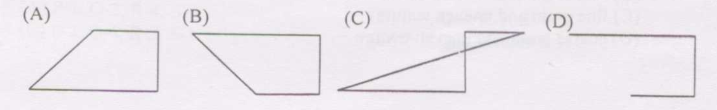
\includegraphics[width=1\linewidth]{figs/fig1.png}
    \caption{}
    \label{fig1}
\end{figure}
 \item  A sector has a gross density of $250$ persons per hectare and a net density of $400$ persons per hectare. If the area of the sector is $120$ hectares,then the percentage of non-residential area is \hfill \textbf{(GATE EE 2025)}
 \begin{enumerate}
 \begin{multicols}{4}
     \item $30$
     \item $35.5$
     \item $37.5$
     \item $40$
     \end{multicols}
 \end{enumerate}
 \item Match the \textbf{systems of plumbing} for building drainage in Group I with their \textbf{descriptions} in Group II. \hfill \textbf{(GATE EE 2025)}
 \newline
 \begin{tabular}{p{0.4\textwidth}p{0.5\textwidth}}
  Group I    & Group II  \\
 P. One-pipe system     &1. Minimum two pipes,one for soil and the other for sullage\\
 Q. Two-pipe system & 2. Single pipe for soil and sullage, and serving as vent for all traps\\
 R. single stack system &3. Minimum two pipes,one for soil and sullage and other for vent\\
   &4. Single pipe for soil and sullage,and serving as vent for soil traps only\\
 \end{tabular}
\begin{enumerate}
\begin{multicols}{2}
  \item P-4,Q-3,R-2
  \item P-3,Q-2,R-1
  \item P-2,Q-3,R-4
  \item P-3,Q-1,R-2
    
\end{multicols}
\end{enumerate}
\item In a plane truss,the equation in terms of \textbf{m} and \textbf{j} is used to check its determinacy and stability ,where \textbf{m} = number of members and \textbf{f} = number of joints. The truss is deficient and unstable when \hfill \textbf{(GATE EE 2025)}
\begin{enumerate}
    \item $m<2j-3$
    \item $m = 2j-3$
    \item $m > 2j-3$
    \item both (A) and (B) are correct
\end{enumerate}
\item Match the \textbf{functions} in Group I with the \textbf{numbers} shown in the given figure of Concentric Zone Theory by Burgress. \hfill \textbf{(GATE EE 2025)}
\newline
\begin{figure}[h]
    \centering
    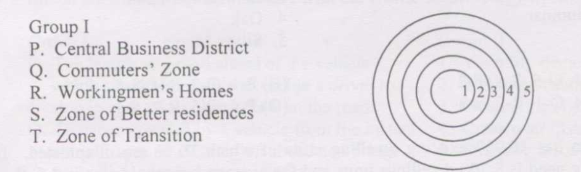
\includegraphics[width=0.6\linewidth]{figs/fig2.png}
    \caption{}
    \label{fig2}
\end{figure}
\begin{enumerate}
    \begin{multicols}{2}
        \item P-1,Q-2,R-5,S-4,T-3
        \item P-1,Q-5,R-3,S-4,T-2
        \item P-2,Q-4,R-5,S-3,T-1
        \item P-3,Q-5,R-1,S-4,T-2
    \end{multicols}
\end{enumerate}
\item For a PERT activity,the optimistic time,most likely time and pessimistic time are $1$,$2$ and $9$ days respectively.The expected time for the activity(in days) is \hfill \textbf{(GATE EE 2025)}
\begin{enumerate}
\begin{multicols}{4}
    \item $9$
    \item $6$
    \item $4$
    \item $3$
\end{multicols}
\end{enumerate}
\item Zoning regulations deal with \hfill \textbf{(GATE EE 2025)}
\newline
  \begin{tabular}{p{0.4\textwidth}p{0.5\textwidth}}
P. Density     & S. Minimum areas of rooms \\
Q. Land use    & T. Height\\
R. Building materials&U. Reserved land areas\\
\end{tabular}
\begin{enumerate}
\begin{multicols}{4}
    \item P,Q,T
    \item P,Q,R,U
    \item Q,S,U
    \item Q,R,S,T
\end{multicols}
\end{enumerate}
\item Match the \textbf{temples} in Group I with their \textbf{distinguishing features} in Group II.\hfill \textbf{(GATE EE 2025)}
\newline
\begin{tabular}{p{0.4\textwidth}p{0.5\textwidth}}
Group I     & Group II \\
P. Konark     & 1. Golden lily Pond\\
Q. Madhurai &2. Sculptured Marble Ceiling\\
R. Dilwara & 3. Twin Vimanas\\
S. Mamallapuram & 4. Chariot\\
  & 5. Torana\\
\end{tabular}
\begin{enumerate}
\begin{multicols}{2}
    \item P-3,Q-1,R-2,Q-5
    \item P-4,Q-1,R-2,S-3
    \item P-2,Q-3,R-5,S-1
    \item P-3,Q-4,R-1,S-2
\end{multicols}
\end{enumerate}
\item The correct sequence of  generic elements in a \textbf{Classical order} arranged from top to bottom is \hfill \textbf{(GATE EE 2025)}
\begin{enumerate}
    \item $\text{Architrave} \longrightarrow\text{Frieze}\longrightarrow\text{Capital}\longrightarrow\text{Cornice}\longrightarrow\text{Shaft}\longrightarrow\text{Pedestal}\longrightarrow\text{Base}$
    \item $\text{Architrave}\longrightarrow\text{Capital}\longrightarrow\text{Cornice}\longrightarrow\text{Frieze}\longrightarrow\text{Base}\longrightarrow\text{Shaft}\longrightarrow\text{Pedestal}$
    \item $\text{Cornice}\longrightarrow\text{Frieze}\longrightarrow\text{Architrave}\longrightarrow\text{Capital}\longrightarrow\text{Shaft}\longrightarrow\text{Base}\longrightarrow\text{Pedestral}$
    \item $\text{Cornice}\longrightarrow\text{Capital}\longrightarrow\text{Frieze}\longrightarrow\text{Architrave}\longrightarrow\text{Shaft}\longrightarrow\text{Pedestral}\longrightarrow\text{Base}$
\end{enumerate}
\item  Match the \textbf{tree forms} in Group I with their \textbf{common examples} in Group II.\hfill \textbf{(GATE EE 2025)}
\newline
\begin{tabular}{p{0.4\textwidth}p{0.5\textwidth}}
  Group I   & Group II \\
 P. Broad    & 1. False Acacia\\
 Q. Tapering & 2. Holly\\
 R. Conical & 3. Lombardy Poplar\\
 S. Columnar & 4. Oak\\
   & 5. Silver Maple\\
\end{tabular}
\begin{enumerate}
\begin{multicols}{2}
    \item P-1,Q-5,R-4,S-2
    \item P-1,Q-3,R-4,S-5
    \item P-2,Q-3,R-4,S-1
    \item P-3,Q-4,R-1,S-2
\end{multicols}
\end{enumerate}
\item A town has $16,000$ existing dwellings units of which $10\%$ are dilapidated. If the housing need is $8,700$ dwellings units and the average household size is $4.5$, then the population of the town is \hfill \textbf{(GATE EE 2025)}
\begin{enumerate}
\begin{multicols}{4}
    \item $64,800$
    \item $1,03,950$
    \item $1,11,150$
    \item $1,18,350$
\end{multicols}
\end{enumerate}
\item Match the \textbf{descriptions} in Group I with the elements of \textbf{Orientation} in Group II. \hfill \textbf{(GATE EE 2025)}
\newline
\begin{tabular}{p{0.6\textwidth}p{0.5\textwidth}}
Group I     & Group II \\
P. Painting on a freshly spread moist plaster surface with powdered pigments     & 1. Chiaroscuro\\
Q. Figure incised into a stone surface or a metal plate yeilding an impression in relief & 2. Emboss\\
R. Delicate or intricate design on lattice work allowing light through oenings & 3. Filigree\\
S. Artistic composition consisting of motifs borrowed from different sources & 4. Fresco\\
  & 5. Intaglio\\
  &6. Pastiche\\
\end{tabular}
\begin{enumerate}
\begin{multicols}{2}
    \item P-6,Q-5,R-1,S-2
    \item P-1,Q-3,R-5,S-2
    \item P-6,Q-3,R-1,S-4
    \item P-5,Q-6,R-3,S-4
\end{multicols}
\end{enumerate}
\item  Match the \textbf{city plans} in Group I with their \textbf{designers} in Group II.
\newline
\begin{tabular}{p{0.4\textwidth}p{0.5\textwidth}}
Group I     & Group II \\
P. London     & 1. Eliel Saarinen\\
Q. Berlin & 2. Kenzo Tange\\
R. Helsinki & 3. Alvar Aalto\\
S. Tokyo & 4. Tadao Ando\\
  & 5. Martin Machler\\
  & 6. Patrick Abercrombie\\
\end{tabular}
\begin{enumerate}
\begin{multicols}{2}
    \item P-6,Q-5,R-1,S-2
    \item P-1,Q-3,R-5,S-2
    \item P-6,Q-3,R-1,S-4
    \item P-5,Q-6,R-4,S-3
\end{multicols}
\end{enumerate}
\item  On a door opening with effective span L,the total weight(W) of an equilateral triangle on the base L is considered as a uniformly distributed load over the span. The bending moment for the door opening is given by \hfill \textbf{(GATE EE 2025)}
\begin{enumerate}
\begin{multicols}{4}
    \item $WL/2$
    \item $WL/4$
    \item $WL/6$
    \item $WL/8$
\end{multicols}
\end{enumerate}
\item  Match the \textbf{descriptions} in Group I with the \textbf{traffic terminology} in Group II. \hfill \textbf{(GATE EE 2025)}
\newline
\begin{tabular}{p{0.6\textwidth}p{0.5\textwidth}}
P. The length of a r
oad ahead of the vehicle which should be visible to enable a driver to stop in case of an obstruction on the road     & 1. Visibility distance \\
Q. Distance covered by a vehicle from the instant a driver sees an obstruction ahead and brings the vehicle to a stop     & 2. Sighting distance\\
R. Distance required for a vehicle to overtake and safely pass another vehicle moving in the same direction but at a lower speed & 3. Overtaking sight distance\\
  & 4. Cross over distance\\
   &5. Stopping distance\\
\end{tabular}
\begin{enumerate}
\begin{multicols}{2}
    \item P-1,Q-3,R-4
    \item P-4,Q-3,R-5
    \item P-2,Q-5,R-4
    \item P-2,Q-5,R-3
\end{multicols}
\end{enumerate}
\item Match the \textbf{labels} on a panelled door in Group I with their \textbf{names} in Group II. \hfill \textbf{(GATE EE 2025)}
\begin{figure}[h]
    \centering
    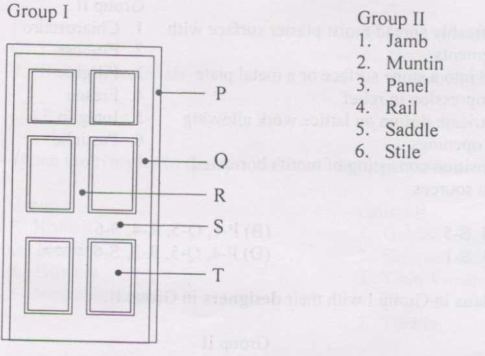
\includegraphics[width=0.6\linewidth]{figs/fig3.png}
    \caption{}
    \label{fig3}
\end{figure}
\begin{enumerate}
    \begin{multicols}{2}
        \item P-1,Q-6,R-5,S-4,T-2
        \item P-1,Q-6,R-2,S-4,T-3
        \item P-5,Q-3,R-1,S-6,T-2
        \item P-5,Q-6,R-1,S-4,T-3
    \end{multicols}
\end{enumerate}
\item A house was constructed $20$ years ago at a cost of Rs. $1,00,000$. The estimated life of the buiding is $50$ years,at the end of which it will have a $15\%$ scrap value of its cost of constuction.Its present value in Rupees is \hfill \textbf{(GATE EE 2025)}
\begin{enumerate}
\begin{multicols}{4}
    \item $36,000$
    \item $66,000$
    \item $75,000$
    \item $85,000$
\end{multicols}
\end{enumerate}
\item A typical roof top \textbf{Rainwater Harvesting System} essentially comprises of \hfill \textbf{(GATE EE 2025)}
\newline
P. Roof catchment
\newline
Q. Down pipes
\newline
R. Rain guage
\newline
S. Filter chamber
\newline
\begin{enumerate}
\begin{multicols}{4}
    \item P,R
    \item P,R,S
    \item Q,R,S
    \item P,Q,S
\end{multicols}
\end{enumerate}
\item Match the \textbf{architects} in Group I with their \textbf{works} in Group II.\hfill \textbf{(GATE EE 2025)}
\newline
\begin{tabular}{p{0.4\textwidth}p{0.5\textwidth}}
Group I     & Group II \\
P. Norman Foster     & 1. Petronas towers\\
Q. Cesar Pelli & 2. Kansai Airport\\
R. Richard Meier & 3. HSBC,Hongkong\\
S. Renzo Piano & 4. The Atheneum\\
  & 5. Sydney Opera House\\
\end{tabular}
\begin{enumerate}
\begin{multicols}{2}
    \item P-3,Q-1,R-4,S-2
    \item P-4,Q-1,R-2,S-3
    \item P-3,Q-2,R-5,S-1
    \item P-5,Q-3,R-1,S-2
\end{multicols}
\end{enumerate}
  
\item A single room of $3 \quad meters  \times 5 \quad meters$ meters enclosed by $20$ cm thick walls has to be constructed.The required foundation trench is $80$ cm wide and $80$ cm deep. The quantity of earthwork in excavation in cubic meters is \hfill \textbf{(GATE EE 2025)}
\begin{enumerate}
\begin{multicols}{4}
    \item $10.75$
    \item $12.80$
    \item $18.70$
    \item $20.24$
\end{multicols}
\end{enumerate}
\item Match the parts of a \textbf{tree log} in Group I with their \textbf{descriptions} in Group II.\hfill \textbf{(GATE EE 2025)}
\newline
\begin{tabular}{p{0.4\textwidth}p{0.5\textwidth}}
Group I     & Group II \\
P. Heartwood     & 1. Outer annual rings of the tree\\
Q. Sapwood & 2. Thin horizontal veins radiating from the pith towards the bark\\
R. Cambium Layer & 3. Outermost protective covering of the log\\
S. Medullary Rays & 4. Innermost rings surroundings the pith\\
    & 5. Outermost one ring between the bark and sapwood\\
\end{tabular}
\begin{enumerate}
\begin{multicols}{2}
    \item P-4 ,Q-2 ,R-5 ,S-3
    \item P-3 ,Q-5 ,R-4 ,S-1
    \item P-4 ,Q-1 ,R-5 ,S-2
    \item P-5 ,Q-1 ,R-4 ,S-2
\end{multicols}
\end{enumerate}
\item  The quantity of plastering in sq.m required for both sides of a wall $5.0 \quad m \times 0.3 \quad m \times 3.0 \quad m$ ($L \times B \times  H$) with a window opening $2.0m \times 0.30m \times 1.2 m$ is \hfill \textbf{(GATE EE 2025)}
\begin{enumerate}
\begin{multicols}{4}
   \item $25.2$
    \item $27.6$
    \item $30.0$
    \item $34.8$
\end{multicols}
\end{enumerate}
\item Match the \textbf{Urban Theorists} in Group I with the \textbf{Planning concepts} in Groups II.\hfill \textbf{(GATE EE 2025)}
\newline
\begin{tabular}{p{0.4\textwidth}p{0.5\textwidth}}
Group I     & Group II \\
P. Patrick Geddes     & 1. Cities in evolution and their relationship with man\\
Q. Charles Abrams  & 2. Judicious use of  technological power\\
R. Constantine Doxiadis & 3. Role of housing in urban development\\
S. Lewis Mumford & 4. The science of human settlements called Ekistics\\
\end{tabular}
\begin{enumerate}
\begin{multicols}{2}
    \item P-1,Q-3,R-4,S-2
    \item P-4,Q-2,R-3,S-1
    \item P-3,Q-4,R-1,S-2
    \item P-2,Q-1,R-4,S-3
\end{multicols}
\end{enumerate}
\item If the reinforcement steel provided for a RCC slab volume $15.0$ cu.m. is @ $1\%$ then the quality of steel required in kilogram is \hfill \textbf{(GATE EE 2025)}
\begin{enumerate}
\begin{multicols}{4}
    \item $655.5$
    \item $1,000.0$
    \item $1,177.5$
    \item $1,500$
\end{multicols}
\end{enumerate}
\item The \textbf{Prairie House} design of Frank Lloyd Wright is characterised by \hfill \textbf{(GATE EE 2025)}
\newline
P. Horizontal planes
\newline
Q. Extended roofs
\newline
R. Focal fire place
\newline
S. Steel coloumns
\newline
T. Vertical screen windows
\begin{enumerate}
\begin{multicols}{4}
    \item P,R,S
    \item P,Q,S
    \item Q,R,S,T
    \item P,Q,R,T
\end{multicols}
\end{enumerate}
  
\item Match the \textbf{window types} in Group I with their \textbf{descriptions} in Group II. \hfill \textbf{(GATE EE 2025)}
\newline
\begin{tabular}{p{0.4\textwidth}p{0.5\textwidth}}
  Group I   & Group II \\
P. Bay window     & 1. Horizontal louvers pivoting simultaneously in a common frame\\
Q. Pivoted window & 2. A sash that rotates $90^\circ$ or $180^\circ$ about a vertical or horizontal axis at or near its centre\\
R. Dorner window & 3. Projecting outward from the main wall of a building,forming an alcove within a room.\\
  & 4. Vertical window projecting out of a sloping roof\\
\end{tabular}
\begin{enumerate}
\begin{multicols}{2}
    \item P-3,Q-2,R-4
    \item P-2,Q-3,R-1
    \item P-1,Q-4,R-2
    \item P-4,Q-2,R-3
\end{multicols}
\end{enumerate}
\item Match the \textbf{Housing projects} in Group I with the \textbf{architects} in Group II.
\newline
\begin{tabular}{p{0.5\textwidth}p{0.5\textwidth}}
  Group I   & Group II \\
  P. Tara Group Housing,New Delhi   &1. Balkrishna Doshi\\
  Q. Marine Front Housing,Cochin &2. Charles Correa\\
  R. Aranya Community Housing,Indore &3. Hasmukh Patel\\
  S. Asiad village,New Delhi &4. Kuldip Singh\\
     & 5. Laurie Baker\\
      &6. Raj Rewal\\
\end{tabular}
\begin{enumerate}
    \begin{multicols}{2}
        \item P-2,Q-4,R-1,S-6
        \item P-3,Q-4,R-2,S-6
        \item P-2,Q-5,R-6,S-1
        \item P-1,Q-5,R-3,S-6
    \end{multicols}
\end{enumerate}
\item A beam of $50$ mm diameter is simply supported at both ends and has an effective span of $6$ meters. It carries two loads of $50$ kN each at one-third span. The section modulus (in cubic cm) of the beam at the quarter span is \hfill \textbf{(GATE EE 2025)}
\begin{enumerate}
\begin{multicols}{4}
    \item $11.17$
    \item $12.27$
    \item $13.37$
    \item $14.47$
\end{multicols}
\end{enumerate}
\item Match the \textbf{Earthqake related terms} in Group I with their \textbf{definitions} in Group II.\hfill \textbf{(GATE EE 2025)}
\newline
\begin{tabular}{p{0.4\textwidth}p{0.5\textwidth}}
 Group I    & Group II \\
P. Focus     & 1. The geographical point on the earth's surface vertically above the originating source\\
Q. Epicentre & 2. The originating source of the seismic waves inside the earth\\
R. Centre of Mass & 3. The point corresponding to the centre of gravity of a structural system\\
S. Centre of Stiffness & 4. The point through which the resultant of the restoring forces of a structural system act\\
\end{tabular}
\begin{enumerate}
\begin{multicols}{2}
    \item P-1,Q-2,R-3,S-4
    \item P-1,Q-2,R-4,S-3
    \item P-2,Q-1,R-3,S-4
    \item P-2,Q-1,R-4,S-3
\end{multicols}
\end{enumerate}
  
\item Match the \textbf{architectural styles} in Group I with the \textbf{construction system} in Group II.\hfill \textbf{(GATE EE 2025)}
\newline
\begin{tabular}{p{0.4\textwidth}p{0.5\textwidth}}
Group I & Group II\\
P. Greek     & 1. Semi-circular arch \\
Q. Roman     & 2. Trabeation\\
R. Indian  & 3. Corbelling\\
S. Gothic  & 4. Pointed arch\\
\end{tabular}
\begin{enumerate}
\begin{multicols}{2}
    \item P-2,Q-4,R-3,S-1
    \item P-1,Q-2,R-4,S-3
    \item P-2,Q-1,R-3,S-4
    \item P-3,Q-1,R-2,S-4
\end{multicols}
\end{enumerate}
\item For incandescent lamps the distributions of total energy emission is \hfill \textbf{(GATE EE 2025)}
\begin{enumerate}
    \item $5\%$ light \& $95\%$ heat
    \item $25\%$ light \& $75\%$ heat
    \item $50\%$ light \& $50\%$ heat
    \item $75\%$ light \& $25\%$ heat
\end{enumerate}
\item Match the \textbf{characteristics} in Group I with the \textbf{climate types} in Group II.\hfill \textbf{(GATE EE 2025)}
\newline
\begin{tabular}{p{0.5\textwidth}p{0.5\textwidth}}
Group I     & Group II \\
P. High humidity accelerates rusting and rotting     & 1. Composite or monsoon\\
Q. High daytime temparature and rapid cooling at night cause materials to crack & 2. Hot dry desert\\
R. Seasonal changes in relative humidity cause rapid weakening of building materials & 3. Hot dry maritime\\
  & 4. Tropical Upland\\
  & 5. Warm humid\\
\end{tabular}
\begin{enumerate}
\begin{multicols}{2}
    \item P-5,Q-2,R-1
    \item P-4,Q-1,R-3
    \item P-5,Q-3,R-4
    \item P-4,Q-3,R-5
\end{multicols}
\end{enumerate}
\item The Architectural projects of the \textbf{International Style} are \hfill \textbf{(GATE EE 2025)}
\newline
P. Aurora House by Aldo Rossi
\newline
Q. Schroder House by Gerrit Reitveid
\newline
R. Thematic House by Jencks \& Farrell
\newline
S. Tugendhat House by Mies vander Rohe
\newline
T. Villa Savoye by Le Corbusier
\begin{enumerate}
\begin{multicols}{4}
    \item P,Q,R,T
    \item P,S
    \item Q,S,T
    \item Q,R,T
    \end{multicols}
\end{enumerate}
\item Tactile flooring with guiding blocks,an element of Barrier Free Design,is used to aid \hfill \textbf{(GATE EE 2025)}
\newline
P. ambulant disabled
\newline Q. non-ambulant disabled \newline  R. partially sighted \newline S. totally blind \begin{enumerate}
\begin{multicols}{4}
    \item P,Q,S \item P,Q,R \item R,S \item Q,S
    \end{multicols}
\end{enumerate}
  
\item Match the \textbf{characteristics of vaults} in Group I with their \textbf{names} in Group II.\hfill \textbf{(GATE EE 2025)}
\newline
\begin{tabular}{p{0.4\textwidth}p{0.5\textwidth}}
Group I     &Group II  \\
P. Uniform semi-circular cross section     & 1. Barrel\\
Q. Semi-circular cross section larger at one end than the other & 2. Cloister\\
R. Compound vault formed by perpendicular intersection of two vaults & 3. Conical\\
S. Compound vault formed by four coves meeting along diagonal vertical planes & 4. Groin\\
  & 5. Rampant\\
  &6. Stilted\\
\end{tabular}
\begin{enumerate}
\begin{multicols}{2}
    \item P-1,Q-6,R-5,S-2
    \item P-6,Q-3,R-4,S-2
    \item P-4,Q-5,R-2,S-6
    \item P-1,Q-3,R-4,S-2
\end{multicols}
\end{enumerate}
\item  A $60^\circ$ segmental arch is provided over a door of $1.0$ m width.The wall thickness is $30$ cm and the arch thickness is $20$ cm. The mean length of the arch in meters is \hfill \textbf{(GATE EE 2025)}
\begin{enumerate}
\begin{multicols}{4}
    \item $1.00$
    \item $1.15$
    \item $1.20$
    \item $1.30$
    \end{multicols}
\end{enumerate}
\item Match the statements about \textbf{elevators \& esclators} in Group I with \textbf{True/False} in Group II.\hfill \textbf{(GATE EE 2025)}
\newline
\begin{tabular}{p{0.5\textwidth}p{0.5\textwidth}}
Group I  &  Group II\\
P. Handling capacity of elevators for residential buildings as per Indian standards is $7.5\%$      &  1. True\\
Q. Minimum height from the top floor to the bottom of the lift machine room should be $3,000$ mm     & 2. False\\
R. Minimum width for escalators as per Indian standards is $1,000$ mm & \\
S. Recommended angle with the horizontal for escalators is $30^\circ$  &  \\
\end{tabular}
\begin{enumerate}
\begin{multicols}{2}
    \item P-1,Q-2,R-1,S-2
    \item P-2,Q-2,R-2,S-1
    \item P-2,Q-1,R-1,S-1
    \item P-1,Q-2,R-2,S-1
    \end{multicols}
\end{enumerate}
\item The slenderness ratio for a cantilever prismatic column of length \textbf{L} with a circular cross section having radius \textbf{r} is \hfill \textbf{(GATE EE 2025)} 
\begin{enumerate}
\begin{multicols}{4}
    \item $L/r$
    \item $2L/r$
    \item $3L/r$
    \item $4L/r$
    \end{multicols}
\end{enumerate}
\item Match the \textbf{designers} in Group I with the \textbf{terms} in Group II. \hfill \textbf{(GATE EE 2025)}
\newline
\begin{tabular}{p{0.4\textwidth}p{0.5\textwidth}}
Group I     & Group II \\
P. Max Dubois     & 1. Prefabrication\\
Q. Joseph Paxton & 2. Domino System\\
R. Victor Horta & 3. Minimalism\\
   & 4. Vegetal Ornamentation\\
   \end{tabular}
\begin{enumerate}
 \begin{multicols}{2}
    \item P-2,Q-1,R-4
    \item P-4,Q-1,R-3
    \item P-2,Q-4,R-3
    \item P-1,Q-3,R-4
\end{multicols}
\end{enumerate}
  
\begin{center}
    \textbf{Common Data Questions}
\end{center}
\textbf{Common Data for Questions 71,72,73}
\newline
The continuous utility data for a construction project is as follows:
\newline
    \begin{tabular}{c c c c}
\textbf{Activity}& \multicolumn{2}{c } {\textbf{Duration(days)}}
         & \textbf{Immediate Predecessors}\\
\cline{2-3}
& Normal & crash & \\ 
P & 3 & 3 & - \\
Q & 4 & 4 & P\\
R & 2 & 1 & P\\
S & 3 & 3 & P\\
T & 0 & 0 & Q\\
U & 6 & 5 & R,T\\
V & 4 & 2 & S\\
\end{tabular}
\newline
\item The normal project time for the given network is \hfill \textbf{(GATE EE 2025)}
\begin{enumerate}
\begin{multicols}{4}
    \item $11$ \item $12$ \item $13$ \item $14$
    \end{multicols}
\end{enumerate}
\item For the all normal soltion, the total float and free float for the activity S are \hfill \textbf{(GATE EE 2025)} 
\begin{enumerate}
\begin{multicols}{4}
    \item $1,1$
    \item $0,3$
    \item $3,3$
    \item $3,0$
    \end{multicols}
\end{enumerate}
\item While crashing the project, the first step of compression would involve the activity \hfill \textbf{(GATE EE 2025)}
\begin{enumerate}
\begin{multicols}{4}
    \item R \item U \item T \item V
    \end{multicols}
    \end{enumerate}
\textbf{Common Data for Questions 74,75:}
\newline
A room measuring $10 \quad m \times 10 \quad m$  has to be illuminated to a level of $200$ lux by a single electrical lamp. The coefficient of utilization is $0.75$ and the maintenance factor is $0.8$.
\newline
\item The lumen output required for the above lamp is \hfill \textbf{(GATE EE 2025)}
\begin{enumerate}
\begin{multicols}{4}
\item $12,000$
\item $16,666$
\item $30,000$
\item $33,333$
\end{multicols}
\end{enumerate}
\item The depreciation factor for the above lamp is \hfill\textbf{(GATE EE 2025)}
\begin{enumerate}
\begin{multicols}{4}
    \item $0.6$
    \item $1.25$
    \item $1.33$
    \item $1.66$
    \end{multicols}
\end{enumerate}
  
\begin{center}
    \textbf{Linked Answer Question: Q.76 to Q.85 carry two marks each}
\end{center}
\textbf{Statement for Linked Answer Questions 76 \& 77:}
\newline
The following data is related to the design of a septic tank for a housing complex:
\newline
Population of housing complex = $150$ \newline
Water supply/person/day = $130$ litres \newline
Waste water flow = $80\%$ of water supply \newline
Detention period = $1$ day \newline
Sludge production = $0.045$ cu.m / person /year \newline Storage capacity for sludge = $\frac{1}{3}^\text{rd}$ of specific tank capacity
\newline
\item Total capacity of septic tank in cubic metres is \hfill\textbf{(GATE EE 2025)}
\begin{enumerate}
\begin{multicols}{4}
    \item $31.70$
    \item $23.40$
    \item $20.80$
    \item $15.60$
\end{multicols}
\end{enumerate}
\item De-sludging interval (to the nearest year) is \hfill\textbf{(GATE EE 2025)}
\begin{enumerate}
    \begin{multicols}{4}
        \item $1$
        \item $2$
        \item $3$
        \item $4$
    \end{multicols}
\end{enumerate}
\textbf{Statement for Linked Answer Questions 78 \& 79:}
\newline
A residential plot measuring $12 \quad meters \times 15 \quad metres $abuts a road on its smaller side. Permissible ground coverage =$50\%$, Floor Space Index (FSI) = $2.5$ and maximum permisible floors = $4$
\newline
\item Maximum total buildable area in sq.m is \hfill\textbf{(GATE EE 2025)}
\begin{enumerate}
    \begin{multicols}{4}
        \item $180$ 
        \item $225$
        \item $360$
        \item $450$
    \end{multicols}
\end{enumerate}
\item As per revised buiding bye-laws,if the required setbacks are - Front $3$ metres, each side $2$ metres and Rear $2$ metres, then the maximum total buildable area will \hfill\textbf{(GATE EE 2025)}
\begin{enumerate}
    \begin{multicols}{2}
        \item increases by $248 \text{sq.m}$
        \item increases by $40 \text{sq.m}$
        \item decreases by $30 \text{sq.m}$
        \item decreases by $40 \text{sq.m}$
    \end{multicols}
\end{enumerate}
\textbf{Statement for Linked Answer Questions 80 \& 81:}
\newline
An aeriel photograph is taken from a plane with a camera lens of focal length $305$ mm. The desired scale of photograph is $1:25,000$ and the height of the terrian above mean sea level is $300$ metres.
\newline
\item The flying height of the plane above mean sea level is \hfill\textbf{(GATE EE 2025)}
\begin{enumerate}
    \begin{multicols}{4}
        \item $7,625$ \item $7,925$ \item $8,562$ \item $8,965$
    \end{multicols}
\end{enumerate}
\item If the above photograph is taken by a camera lens of focal length $210$ mm from the same flying height, then the scale of the photograph will be \hfill\textbf{(GATE EE 2025)}
\begin{enumerate}
    \begin{multicols}{4}
        \item $1:45,000$ \item $1:37,740$ \item $1:36,310$ \item $1:19,050$
    \end{multicols}
\end{enumerate}
  
\textbf{Statements for Linked Answer Questions 82 \& 83:}
\newline
A beam of cross section $300 \quad mm \times 400 \quad mm$ has overhangs at both ends. The beam has a simple support of $10 \text{meters}$ and an overhang of $5 \text{meters}$ each at both ends and carrying a load of $10 \text{kN}$ on both the free ends.
\newline
\item The maximum values of shear force and bending moment in the beam are \hfill\textbf{(GATE EE 2025)}
\begin{enumerate}
    \begin{multicols}{2}
        \item $5 \text{kN}$ , $50 \text{kN-m}$
        \item $20 \text{kN}$ , $80 \text{kN-m}$
        \item $15 \text{kN}$ , $45 \text{kN-m}$
        \item $10 \text{kN}$ , $50 \text{kN-m}$
    \end{multicols}
\end{enumerate}
\item The maximum values of bending stress and shear stress developed in the beam in $N/mm^2$ are \hfill\textbf{(GATE EE 2025)}
\begin{enumerate}
    \begin{multicols}{4}
        \item $5.15$ , $0.1$
        \item $6.25$ ,$0.125$
        \item $7.35$ ,$0.15$
        \item $8.45$ , $0.175$
    \end{multicols}
\end{enumerate}
\textbf{Statements for Linked Answer Questions 84 \& 85:}
An auditorium has a volume of $3000$ $m^3$ with optimum reverberation time of $0.8$ seconds.
\newline
\item The sound absorption power required in the auditorium in $m^2$ -sabins is approximately \hfill\textbf{(GATE EE 2025)}
\begin{enumerate}
    \begin{multicols}{4}
        \item $250$ \item $400$ \item $600$ \item $800$
    \end{multicols}
\end{enumerate}
\item  During a convocation programme in the same auditorium, the absorption power increases by $200$ $m^2$ -sabins . The reverberation time in seconds will now be \hfill\textbf{(GATE EE 2025)}
\begin{enumerate}
    \begin{multicols}{4}
        \item $0.4$ \item $0.6$ \item $0.8$ \item $1.2$
    \end{multicols}
\end{enumerate}
\begin{center}
    \textbf{END OF THE QUESTION PAPER}
\end{center}
\end{enumerate}

\end{document}
